% Options for packages loaded elsewhere
% Options for packages loaded elsewhere
\PassOptionsToPackage{unicode}{hyperref}
\PassOptionsToPackage{hyphens}{url}
\PassOptionsToPackage{dvipsnames,svgnames,x11names}{xcolor}
%
\documentclass[
  12pt,
  oneside]{book}
\usepackage{xcolor}
\usepackage[top=30mm,bottom=30mm,left=25mm,right=20mm,headheight=15mm,footskip=33pt]{geometry}
\usepackage{amsmath,amssymb}
\setcounter{secnumdepth}{5}
\usepackage{iftex}
\ifPDFTeX
  \usepackage[T1]{fontenc}
  \usepackage[utf8]{inputenc}
  \usepackage{textcomp} % provide euro and other symbols
\else % if luatex or xetex
  \usepackage{unicode-math} % this also loads fontspec
  \defaultfontfeatures{Scale=MatchLowercase}
  \defaultfontfeatures[\rmfamily]{Ligatures=TeX,Scale=1}
\fi
\usepackage{lmodern}
\ifPDFTeX\else
  % xetex/luatex font selection
\fi
% Use upquote if available, for straight quotes in verbatim environments
\IfFileExists{upquote.sty}{\usepackage{upquote}}{}
\IfFileExists{microtype.sty}{% use microtype if available
  \usepackage[]{microtype}
  \UseMicrotypeSet[protrusion]{basicmath} % disable protrusion for tt fonts
}{}
\usepackage{setspace}
\makeatletter
\@ifundefined{KOMAClassName}{% if non-KOMA class
  \IfFileExists{parskip.sty}{%
    \usepackage{parskip}
  }{% else
    \setlength{\parindent}{0pt}
    \setlength{\parskip}{6pt plus 2pt minus 1pt}}
}{% if KOMA class
  \KOMAoptions{parskip=half}}
\makeatother
% Make \paragraph and \subparagraph free-standing
\makeatletter
\ifx\paragraph\undefined\else
  \let\oldparagraph\paragraph
  \renewcommand{\paragraph}{
    \@ifstar
      \xxxParagraphStar
      \xxxParagraphNoStar
  }
  \newcommand{\xxxParagraphStar}[1]{\oldparagraph*{#1}\mbox{}}
  \newcommand{\xxxParagraphNoStar}[1]{\oldparagraph{#1}\mbox{}}
\fi
\ifx\subparagraph\undefined\else
  \let\oldsubparagraph\subparagraph
  \renewcommand{\subparagraph}{
    \@ifstar
      \xxxSubParagraphStar
      \xxxSubParagraphNoStar
  }
  \newcommand{\xxxSubParagraphStar}[1]{\oldsubparagraph*{#1}\mbox{}}
  \newcommand{\xxxSubParagraphNoStar}[1]{\oldsubparagraph{#1}\mbox{}}
\fi
\makeatother


\usepackage{longtable,booktabs,array}
\newcounter{none} % for unnumbered tables
\usepackage{calc} % for calculating minipage widths
% Correct order of tables after \paragraph or \subparagraph
\usepackage{etoolbox}
\makeatletter
\patchcmd\longtable{\par}{\if@noskipsec\mbox{}\fi\par}{}{}
\makeatother
% Allow footnotes in longtable head/foot
\IfFileExists{footnotehyper.sty}{\usepackage{footnotehyper}}{\usepackage{footnote}}
\makesavenoteenv{longtable}
\usepackage{graphicx}
\makeatletter
\newsavebox\pandoc@box
\newcommand*\pandocbounded[1]{% scales image to fit in text height/width
  \sbox\pandoc@box{#1}%
  \Gscale@div\@tempa{\textheight}{\dimexpr\ht\pandoc@box+\dp\pandoc@box\relax}%
  \Gscale@div\@tempb{\linewidth}{\wd\pandoc@box}%
  \ifdim\@tempb\p@<\@tempa\p@\let\@tempa\@tempb\fi% select the smaller of both
  \ifdim\@tempa\p@<\p@\scalebox{\@tempa}{\usebox\pandoc@box}%
  \else\usebox{\pandoc@box}%
  \fi%
}
% Set default figure placement to htbp
\def\fps@figure{htbp}
\makeatother


% definitions for citeproc citations
\NewDocumentCommand\citeproctext{}{}
\NewDocumentCommand\citeproc{mm}{%
  \begingroup\def\citeproctext{#2}\cite{#1}\endgroup}
\makeatletter
 % allow citations to break across lines
 \let\@cite@ofmt\@firstofone
 % avoid brackets around text for \cite:
 \def\@biblabel#1{}
 \def\@cite#1#2{{#1\if@tempswa , #2\fi}}
\makeatother
\newlength{\cslhangindent}
\setlength{\cslhangindent}{1.5em}
\newlength{\csllabelwidth}
\setlength{\csllabelwidth}{3em}
\newenvironment{CSLReferences}[2] % #1 hanging-indent, #2 entry-spacing
 {\begin{list}{}{%
  \setlength{\itemindent}{0pt}
  \setlength{\leftmargin}{0pt}
  \setlength{\parsep}{0pt}
  % turn on hanging indent if param 1 is 1
  \ifodd #1
   \setlength{\leftmargin}{\cslhangindent}
   \setlength{\itemindent}{-1\cslhangindent}
  \fi
  % set entry spacing
  \setlength{\itemsep}{#2\baselineskip}}}
 {\end{list}}
\usepackage{calc}
\newcommand{\CSLBlock}[1]{\hfill\break\parbox[t]{\linewidth}{\strut\ignorespaces#1\strut}}
\newcommand{\CSLLeftMargin}[1]{\parbox[t]{\csllabelwidth}{\strut#1\strut}}
\newcommand{\CSLRightInline}[1]{\parbox[t]{\linewidth - \csllabelwidth}{\strut#1\strut}}
\newcommand{\CSLIndent}[1]{\hspace{\cslhangindent}#1}



\setlength{\emergencystretch}{3em} % prevent overfull lines

\providecommand{\tightlist}{%
  \setlength{\itemsep}{0pt}\setlength{\parskip}{0pt}}



 


\usepackage{Archivo}
%\usepackage[sc]{mathpazo}

\usepackage[T1]{fontenc}
\usepackage{xcolor}
\usepackage[pages=some]{background}
\usepackage{setspace}
\usepackage[table]{xcolor}
\usepackage{tabularx}
\usepackage[Bjornstrup]{fncychap}
\usepackage{multirow}

% Colors Techtraplastice
\definecolor{Naranja}{HTML}{F69223}
\definecolor{Celeste}{HTML}{3299CC}
\definecolor{Verde}{HTML}{98C601}
\definecolor{Neutro}{HTML}{5E6F75}
\definecolor{Neutro_claro}{HTML}{F1F1F1}

\definecolor{Verde_osc}{RGB}{47,93,80}


% Headers
\usepackage{fancyhdr}
\pagestyle{fancy}          

\fancyhead{}
\fancyfoot{}

\fancyhead[L]{
\includegraphics[height=10mm]{assets/images/logo-TTPCE.png}}
\fancyhead[C]{ }
\fancyhead[R]{\thepage}

\fancyfoot[L]{
\includegraphics[height=8mm]{assets/images/footer-00.png}}
\fancyfoot[C]{}
\fancyfoot[R]{
\includegraphics[height=8mm]{assets/images/EU.png}}



\renewcommand{\headrulewidth}{1pt}
\renewcommand{\headruleskip}{1mm}



\usepackage{pdfpages}
\usepackage{wrapfig}
\usepackage{pgfgantt}
\usepackage{academicons}

\usepackage{worldflags}

% Command
\newcommand{\techtra}{\emph{TechTraPlastiCE }}

\usepackage{tabu}

% \usepackage{sectsty}
% \sectionfont{\scshape}
\usepackage{booktabs}
\usepackage{longtable}
\usepackage{array}
\usepackage{multirow}
\usepackage{wrapfig}
\usepackage{float}
\usepackage{colortbl}
\usepackage{pdflscape}
\usepackage{tabularx}
\usepackage{xltabular}
\usepackage{threeparttable}
\usepackage{threeparttablex}
\usepackage[normalem]{ulem}
\usepackage{makecell}
\usepackage{xcolor}
\makeatletter
\@ifpackageloaded{caption}{}{\usepackage{caption}}
\AtBeginDocument{%
\ifdefined\contentsname
  \renewcommand*\contentsname{Table of contents}
\else
  \newcommand\contentsname{Table of contents}
\fi
\ifdefined\listfigurename
  \renewcommand*\listfigurename{List of Figures}
\else
  \newcommand\listfigurename{List of Figures}
\fi
\ifdefined\listtablename
  \renewcommand*\listtablename{List of Tables}
\else
  \newcommand\listtablename{List of Tables}
\fi
\ifdefined\figurename
  \renewcommand*\figurename{Figure}
\else
  \newcommand\figurename{Figure}
\fi
\ifdefined\tablename
  \renewcommand*\tablename{Table}
\else
  \newcommand\tablename{Table}
\fi
}
\@ifpackageloaded{float}{}{\usepackage{float}}
\floatstyle{ruled}
\@ifundefined{c@chapter}{\newfloat{codelisting}{h}{lop}}{\newfloat{codelisting}{h}{lop}[chapter]}
\floatname{codelisting}{Listing}
\newcommand*\listoflistings{\listof{codelisting}{List of Listings}}
\makeatother
\makeatletter
\usepackage{pdflscape}
\makeatother
\makeatletter
\makeatother
\makeatletter
\@ifpackageloaded{caption}{}{\usepackage{caption}}
\@ifpackageloaded{subcaption}{}{\usepackage{subcaption}}
\makeatother
\usepackage{bookmark}
\IfFileExists{xurl.sty}{\usepackage{xurl}}{} % add URL line breaks if available
\urlstyle{same}
% fallback for those not using the hyperref driver hyperxmp:
\makeatletter
\@ifundefined{xmpquote}{\newcommand{\xmpquote}[1]{#1}}{}
\makeatother
\hypersetup{
  pdftitle={D3.1 Benchmarking study},
  pdfauthor={Eng. Sandra Ponce (PUCV),~ Prof.~Carlos Carlesi Jara (PUCV), ~ Prof.~Rolando Chamy (PUCV).; PhD. Kelly Henao (Columbus), Cecilia Valdés (Columbus), Daniel Samoilovich (Columbus); Prof.~Fabio Cruz (UL).},
  colorlinks=true,
  linkcolor={Celeste},
  filecolor={Maroon},
  citecolor={Blue},
  urlcolor={Naranja},
  pdfcreator={LaTeX via pandoc}}


\title{D3.1 Benchmarking study}
\author{Eng. Sandra Ponce (PUCV),~ Prof.~Carlos Carlesi Jara (PUCV), ~
Prof.~Rolando Chamy (PUCV). \and PhD. Kelly Henao (Columbus), Cecilia
Valdés (Columbus), Daniel Samoilovich (Columbus) \and Prof.~Fabio Cruz
(UL).}
\date{November 25, 2026}
\begin{document}
  \begin{frontmatter}
  \begin{titlepage}
  % Inspiration: https://nmfs-opensci.github.io/quarto_titlepages_v1/02-titlepages.html
  % This is a combination of Pandoc templating and LaTeX
  % Pandoc templating https://pandoc.org/MANUAL.html#templates
  % See the README for help



  \backgroundsetup{
    scale=1.0,
    angle=0,
    opacity=0.90,
    contents={
      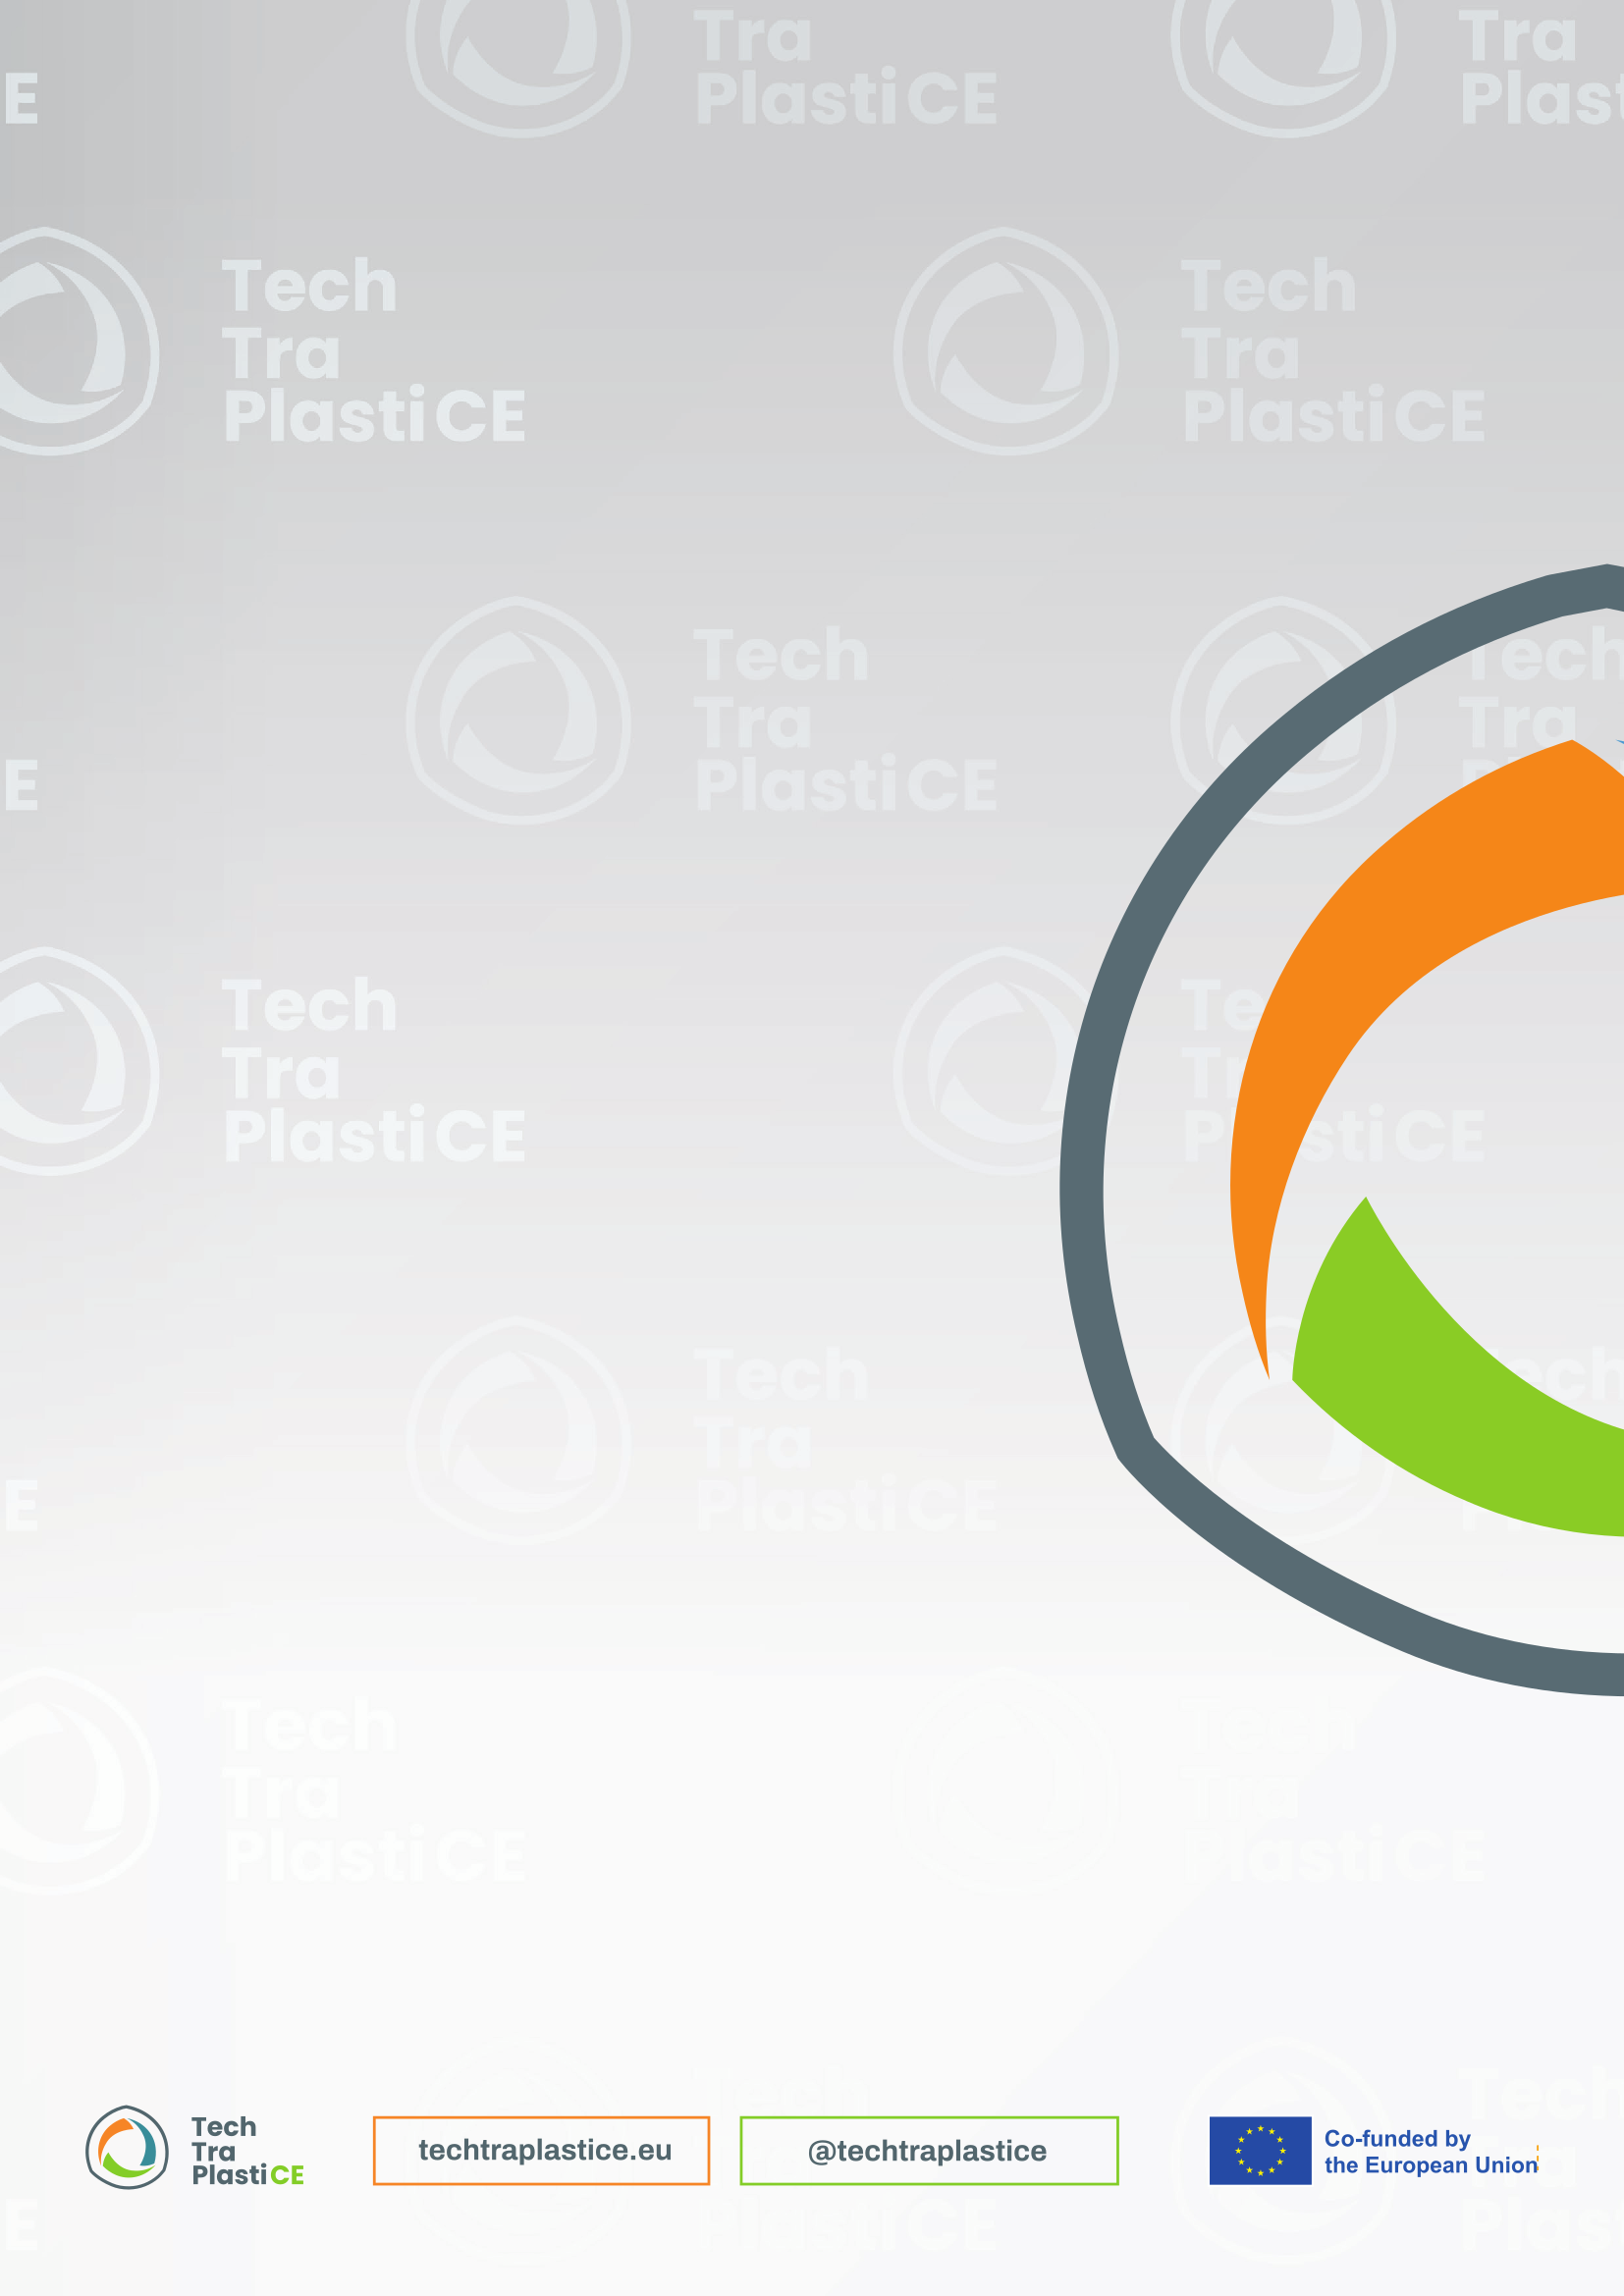
\includegraphics{assets/Portada.png}}
      }

  \BgThispage


  \begin{minipage}[b][0.78\textheight][s]{0.65\textwidth}

    \raggedright
    % Title and subtitle
    
    \vfill

    \begin{spacing}{2.2}
      {\color{Naranja}\Huge\bfseries{D3.1 Benchmarking
  study}} \\[1\baselineskip] 
    \end{spacing}
    
    \begin{spacing}{1.2}
    {\color{Neutro} \Large\textit{WP2: Development of a networked
  portfolio}}\\[1\baselineskip]
    
    {\Large \color{Neutro} 
    Strengthening University Tech Transfer Capabilities to Support Circular Economy 
    Value Chains for Plastics in Latin America -
    \textsc{\centering\bfseries TechTraPlastiCE} }\\[2\baselineskip]

    
    \end{spacing}

    {\color{Neutro} \Large\textit{November 25, 2026}}
    
    \vfill
  \end{minipage}		

  \vfill

  {\scriptsize
    \color{Neutro}
    This project has been funded with the support of Erasmus +.  
    The contents are the responsibility of the author(s). 
    The Commission cannot be held responsible for any use which may be made of the information contained therein. 
    Project No. 101179564 
    }


  \newpage



  \thispagestyle{plain}
  \begin{tabu} to \linewidth {X[1.3,l]  | X[1,l] X[1,l]}
    \toprule
    \multirow{5}{*}{ 
\includegraphics[height=20mm]{assets/images/logo-TTPCE.png}} &  \textbf{Work Package} : & WP2  \\ \cmidrule{2-3}
      & \textbf{Project Number} : & 101179564  \\ \cmidrule{2-3}
      &  \textbf{Type of document}:  & Deliverable   \\ \cmidrule{2-3}
      & \textbf{Due Delivery Date}:    & Nov
  30/2026     \\ \cmidrule{2-3}
      & \textbf{Actual Delivery Date}:    & November 25, 2026       \\ 
    \bottomrule
  \end{tabu}

  \vfill


  \begin{tabu} to \linewidth {X[1,l]  | X[3.5,l]}
    \toprule
    \textbf{Title} : & D3.1 Benchmarking study  \\ \cmidrule{2-2}
    \textbf{Work Package} : & WP2: Development of a networked
  portfolio  \\ \cmidrule{2-2}
    \textbf{Description} : & The identified problems involving
  multi-actors visions and roles are foreseen to be problems that are
  also faced in other countries and cities. The benchmarking will help
  to find inspiration in how similar multilevel problems have been
  approached to start identifying clues of actions. The benchmarking
  study will be structured as a public document available for all the
  partners.  \\ \cmidrule{2-2}
    \textbf{Responsible} : & Pontifica Universida Catolica de Valparaiso
  \& Columbus Association  \\ \cmidrule{2-2}
    \textbf{Author(s)} : &  
     
          Eng. Sandra Ponce (PUCV),~ Prof.~Carlos Carlesi Jara (PUCV), ~
          Prof.~Rolando Chamy (PUCV).
          
          PhD. Kelly Henao (Columbus), Cecilia Valdés (Columbus), Daniel
          Samoilovich (Columbus)
          
          Prof.~Fabio Cruz (UL).
           \\ \cmidrule{2-2}
    \textbf{Project Call} : & ERASMUS-EDU-2024-CBHE (Capacity building in the field of higher education)  \\ \cmidrule{2-2}
    \textbf{Dissemination Level} : & Public\\   
  \bottomrule
  \end{tabu}



  \vfill


  \begin{tabu} to \linewidth {X[0.8,l]  | X[0.7,l] X[0.8,l] X[1.9,l]}
    \toprule
    \textbf{Version}: & \multicolumn{3}{l}{ 1.2} \\ \midrule
    \textbf{Contributors}  & Versions    & Dates       & Revision Description \\ \midrule
    PUCV  & 1    & 13/07/2026  &  First version (19 initiatives).  \\ 
    PUCV  & 2    & 29/10/2026  & Six cases added; updated analysis, revised scope, status, evidence and findings.  \\ 
    COLUMBUS  & 3   & 20/11/2026  & Integration of external report  \\ 
    \bottomrule
\end{tabu}  


    
    
    \vfill
    
    {\scriptsize\centering\color{lightgray} 
    
    Disclaimer
    
    This document is provided <<as is>> with no warranties whatsoever, 
    including any warranty or merchantability, non-infringement, fitness for any particular 
    purpose, or any warranty otherwise arising out of any proposal, specification or sample.  
    
    No license, express or implied, by estoppels or otherwise, to any intellectual 
    property rights are granted herein. 
    The members of the project TechTraPlastiCE do not accept any liability for actions or 
    omissions of TechTraPlastiCE members or third parties and disclaim any obligation 
    to enforce the use of this document. 
    
    This document reflects only the authors' view and the Commission is not responsible 
    for any use that may be made of the information it contains.  
    This document is subject to change without notice. 
    
    }
    \normalsize
    
    
    
      \end{titlepage}
  \end{frontmatter}

\renewcommand*\contentsname{Contents}
{
\setcounter{tocdepth}{2}
\tableofcontents
}
\listoffigures
\listoftables

\setstretch{1.2}
\mainmatter
\chapter*{Executive summary}\label{executive-summary}
\addcontentsline{toc}{chapter}{Executive summary}

This document constitutes the Deliverable \emph{D3.1 -- Benchmarking
Study} of the Work Package 3: « Multi-actor collaborations for just and
safe plastic's circular economy ». The main goal of the document is to
present a comparative analysis of international plastic reuse and
recovery practices. More precisely, this deliverable entails the
development of two TechTraPlastiCE's tasks:

\begin{enumerate}
\def\labelenumi{\arabic{enumi}.}
\tightlist
\item
  \textbf{Task T3.1:} Reuse action clues in Argentina, Chile and
  Colombia
\item
  \textbf{Task T3.3}: Assessment of local reuse systems and benchmarking
  with impactful reuse practices
\end{enumerate}

The scope of this report is twofold. In a first hand, a comprehensive
analysis of the socioeconomic impacts of plastic reuse initiatives in
Argentina, Chile, and Colombia is identified and analyzed including
aspects such as including the state of norms and processes, job
creation, income generation, and economic empowerment, particularly
among marginalized communities. In a second hand, the analysis is
complemented by an exploration of how such challenges have been solved
in other parts of the world (European countries, Africa, etc.) to
inspire action possibilities in preparation for the Search conferences
task and for the development of the Work Package 4 Pilot projects
implementation.

A total of 54 experiences were mapped at the international level.
Particularly, twenty-five initiatives were found in Latin America
--Argentina (9), Chile (10), and Colombia (6)--, based on a tailored
questionnaire for the three countries.

The rest of experiences (29) were mapped at the rest of the world where
information was collected through a specific protocol of analysis. To
better understand, the whole set of experiences were organised into five
families, each recorded in a standardised three-block record sheet and
analysed against the seven-stage recovery chain.

Regarding the experiences found in Argentina, Colombia and Chile, the
total set of experiences cover packaging reuse, plastic-waste collection
and recycling, industrial valorization, and technology development.\\
Twenty-three cases directly address the management, prevention, reuse,
or transformation of plastic waste. Across the three countries, the
cases point to several recurring enabling conditions:

\begin{enumerate}
\def\labelenumi{\arabic{enumi}.}
\tightlist
\item
  Several leviers to impulse the reuse include aspects such as i)
  identified demand for circular products or services, ii) dependable
  material supply, iii) adequate technical and quality standards, iv)
  stakeholder coordination, and vi) financing arrangements suited to the
  operating model.
\item
  Extended Producer Responsibility (EPR) schemes and recycled-content
  requirements can create stable obligations or markets, while public
  procurement and industrial off-take agreements can provide alternative
  demand anchors.
\item
  The existence of regulation, infrastructure, or a validated technology
  is not sufficient on its own. Chilean refilling cases, Argentine
  industrial and municipal cases, and Colombian recycling ventures
  illustrate different vulnerabilities, from commercial dependence and
  dispersed logistics to certification barriers and exposure to
  virgin-material prices.
\item
  The distinction between technological progress, operational scale, and
  long-term viability is central to the findings. Some projects remain
  at research or pilot stage; others operate commercially but face
  financial pressure; still others have closed or were never
  implemented.
\end{enumerate}

On the other hand, from the twenty-nine international experiences, three
cross-cutting findings complemented the perspectives found in Colombia,
Chile:

\begin{enumerate}
\def\labelenumi{(\roman{enumi})}
\tightlist
\item
  the points on `communication' and `separation at source' remain as
  major pain points at the value chain.
\item
  circular economy systems systems that partially fail because of an
  imbalance between push (supply-side) and pull (demand-side) forces.
  Nevertheless, reference systems institutionalise both.
\item
  the sorting and marketing stages concentrate well-designed mechanisms
  with very little independent performance evidence --- a gap in the
  literature that the Deliverable 5 benchmarking can help to fill.
\end{enumerate}

In general, it is recommended that before scaling any resulting reuse
action, it is required to match technologies to real demand, designing
viable logistics and cost-sharing arrangements, validating materials and
market access, including recovery actors appropriately, and testing
resilience. They also identify practical roles for universities as
research partners, independent testing and certification-support
institutions, living laboratories, conveners, and technology-transfer
facilitators.

Overall, the findings provide a comparative understanding of the factors
that shape plastic reuse initiatives in Argentina, Chile, and Colombia.
By identifying common opportunities, recurring barriers, and practical
lessons from both successful and unsuccessful experiences, the study
provides evidence to support decision-making, strengthen stakeholder
collaboration, and inform future circular economy actions in Latin
America.

\chapter{Introduction}\label{introduction}

TechTraPlastiCE project aims to implement multi-actor for just and safe
plastic's circular economy in the context of Colombia, Chile and
Argentina. The identified problems involving multi-actors visions and
roles are foreseen to be problems that are also faced in other countries
and cities. This report aims to establish a benchmarking approach that
will help to find inspiration in how similar multilevel problems have
been approached to start identifying clues of actions. The benchmarking
study will be structured with two major focus:

\begin{enumerate}
\def\labelenumi{\arabic{enumi}.}
\tightlist
\item
  Advances in the reuse challenge in the context of Colombia, Chile and
  Argentina contexts.
\item
  Global benchmarking on strategies in the rest of the world including
  Europe, Africa and other countries of LatinAmerica.
\end{enumerate}

These two perspectives aim to give the TechTraPlastiCE consortium a
baseline of initiatives that have been implemented with a multicriteria
grid lecture. In order to understand the advances, following section
will define the plastic value chain in the frame of circular economy
practices.

\section{Plastic Value Chain at the Circular
Economy}\label{plastic-value-chain-at-the-circular-economy}

The lifecycle of polymer materials can be described by the scheme in
Fig. xx from the extensive polymer science literature {[}Ragaert et al.
(\citeproc{ref-ragaert2017}{2017}); {]}. Five major stages are
considered as follows:

\begin{landscape}

\begin{figure}[H]

{\centering 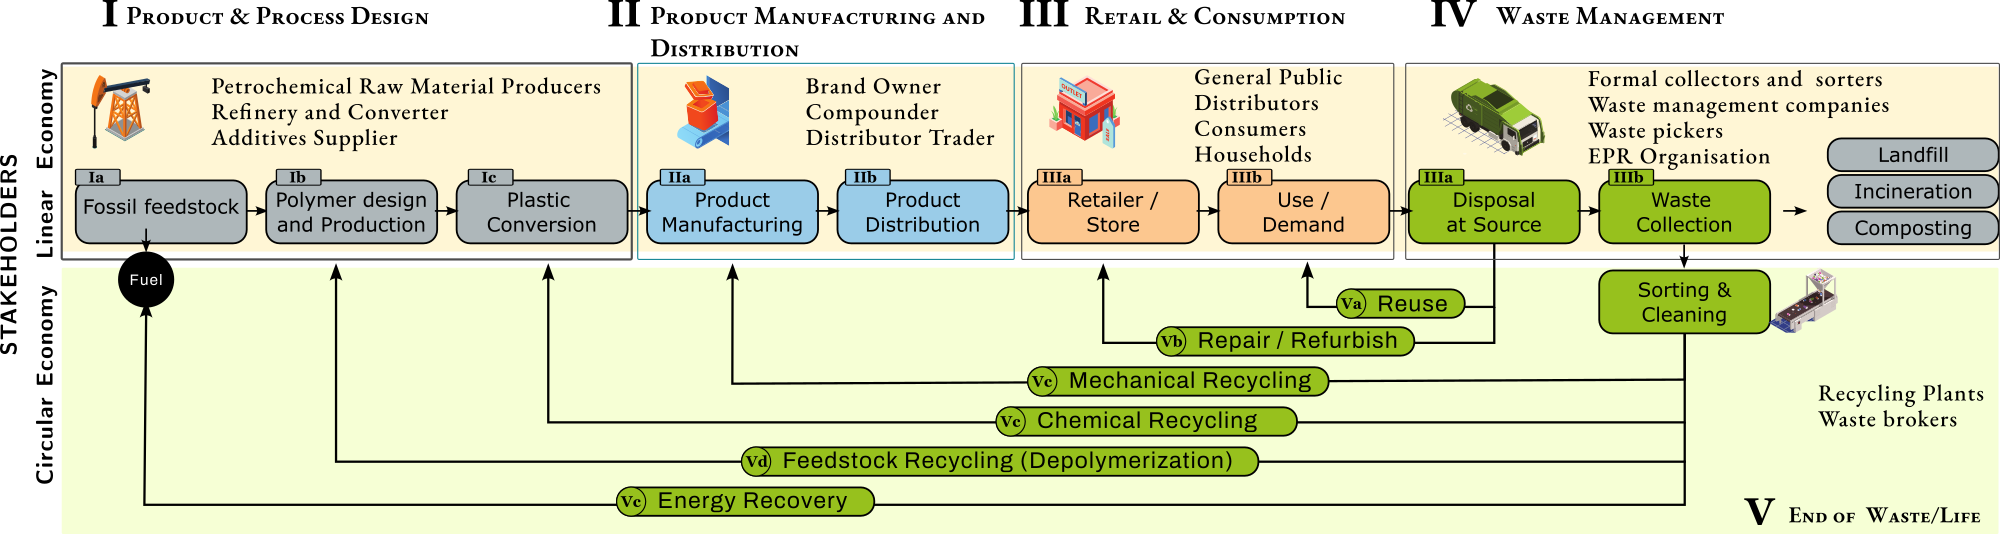
\includegraphics[width=1\linewidth,height=\textheight,keepaspectratio]{figures/3.1/V2.png}

}

\caption{Stakeholders perspective of the Plastic Value Chain for the
Circular Economy}

\end{figure}%

\end{landscape}

\begin{enumerate}
\def\labelenumi{\arabic{enumi}.}
\tightlist
\item
  Product \& Process design,
\item
  Product manufacturing and distribution,
\item
  Retail and consumption,
\item
  Waste Management
\item
  End-of-Waste/life.
\end{enumerate}

The first stage ``I \emph{Product and Process design}'' relates to the
upstream value chain where the raw material producers transform
oil-based products into the different monomers used in the plastic
industry. The primary stakeholder in this stage concerns the plastics
production that refines crude oil and produces monomers that are
chemically bonded into polymers. The different combinations of monomers
and their blending with oxygen, chlorine, fluorine and nitrogen
generates different types of plastics. It is during the design phase
that the function and qualities of the product are decided (e.g.,
colour, recyclability, polymer mix)
(\citeproc{ref-johansen2022}{Johansen et al., 2022}). In this phase most
interactions are built in business to business (B2B).

The Second stage ``Product manufacturing and distribution'' encompasses
the transformation of raw polymer materials into intermediate or
finished plastic products, followed by their transportation and delivery
across supply chains. Manufacturing activities typically involve polymer
processing technologies such as extrusion, injection molding, blow
molding, thermoforming, and other conversion processes, depending on the
intended application and product specifications. This stage involves,
particularly, the industrial actors and logistics providers for the
final and intermediate products. Here business to business (B2B) and
business to consumer (B2C) interactions are mapped. For instance, the
packaging industrial sector remains the largest field of application.

The third stage ``Retail and consumption'' includes the
commercialization, acquisition, utilization, and use of plastic products
by businesses, institutions, and final consumers. It represents the
interface between the production system and the demand side of the
plastic value chain, where purchasing decisions, consumption patterns,
and product-use behaviors influence material demand and subsequent waste
generation. Business to consumer (B2C) interactions are relevant in this
phase.

The fourth stage ``Waste Management'' usually engages the activities and
infrastructure required for the collection, transportation, sorting,
treatment, and recovery of plastic waste generated during manufacturing,
distribution, retail, and consumption. Its primary objective is to
manage discarded plastic materials while minimizing environmental
impacts and maximizing opportunities for resource recovery. In function
of the national context, usually public and public-private partnerships
including municipal authorities, waste collection companies, sorting
facilities, recycling operators, informal waste collectors, and
regulatory institutions. Waste management systems may address both
pre-consumer plastic waste, generated during industrial and commercial
activities, and post-consumer plastic waste, arising after products have
been used and discarded.

Finally, the fifth stage ``End-of-Waste / Life'' encompasses the
activities and infrastructure required for the circular economy actions.
This stage is particularly of the interest of TechTraPlastiCE in terms
because it determines whether discarded plastics are recovered as
secondary resources, converted into energy, permanently disposed of, or
released into the environment. In this state, globally, we can identify
the following strategies :

\begin{itemize}
\tightlist
\item
  \textbf{Reuse:} it refers to the repeated use of plastic products or
  components for their original purpose, without substantial
  modification of their material structure. It may involve collection,
  cleaning, inspection, repair and redistribution operations. By
  extending the service life of products, reuse reduces the demand for
  virgin materials, limits waste generation and avoids the environmental
  impacts associated with the manufacture of new products. Its
  implementation generally requires appropriate product design, reverse
  logistics, consumer participation and economically viable business
  models\textbf{.}
\item
  \textbf{Mechanical recycling}: Mechanical recycling consists of
  recovering and reprocessing plastic waste through physical operations,
  such as sorting, washing, shredding, melting and extrusion, without
  intentionally altering the chemical structure of the polymers. These
  steps may occur in a different order, multiple times depending on the
  origins and composition of the waste. The resulting secondary raw
  materials can be incorporated into the manufacture of new plastic
  products, partially or entirely replacing virgin polymers. However,
  the effectiveness of mechanical recycling depends on the purity and
  homogeneity of waste streams, the presence of contaminants and
  additives, and the degradation of polymer properties during successive
  processing cycles. These limitations may lead to applications with
  lower technical requirements and economic value, a phenomenon commonly
  referred to as \emph{downcycling.}
\item
  \textbf{Chemical recycling}: it encompasses a range of technologies
  that intentionally modify or break down the molecular structure of
  plastic polymers to recover monomers, oligomers or other chemical
  intermediates. Processes such as hydrolysis, glycolysis, methanolysis
  and enzymatic depolymerisation can enable the \emph{production of new
  polymers} with properties comparable to those of virgin materials.
  Chemical recycling can complement mechanical recycling by addressing
  certain waste streams that are difficult to process mechanically.
  Nevertheless, its environmental and economic performance depends on
  energy requirements, chemical consumption, conversion yields,
  technological maturity and the availability of suitable feedstock.
\item
  \textbf{Feedstock recycling}: Feedstock recycling refers to the
  conversion of plastic waste into basic chemical substances or
  hydrocarbon feedstocks that can be reintegrated into industrial
  production processes. Technologies such as pyrolysis, gasification and
  hydrothermal conversion transform polymers into products such as
  pyrolysis oils, synthesis gas or other chemical fractions. Unlike
  selective depolymerisation, feedstock recycling does not necessarily
  seek to recover the original monomers of a specific polymer. It offers
  potential opportunities for the treatment of mixed or contaminated
  plastic waste and the substitution of fossil-based industrial
  feedstocks. Its contribution to material circularity depends, however,
  on the extent to which the recovered substances are used to
  manufacture new materials rather than fuels.
\item
  \textbf{Energy recovery}: Energy recovery involves the conversion of
  the calorific value of plastic waste into useful energy, typically
  through controlled combustion in waste-to-energy facilities or
  co-processing in industrial installations, such as cement kilns.
  Although this strategy can reduce landfill disposal and partially
  substitute conventional energy sources, it results in the irreversible
  loss of the material resources contained in plastics and generates
  greenhouse gas emissions. Consequently, energy recovery is not
  considered a material recycling strategy and occupies a lower position
  in the waste management hierarchy. It is generally regarded as a
  residual treatment option for plastic waste that cannot be reused or
  recycled under technically, economically and environmentally
  acceptable conditions.
\end{itemize}

The different strategies for the circular economy of plastics presents
advantages and challenges given the technological maturity, the
reglamentation aspects and the stakeholders involved. This is why the
goal of this report is to present an overview of the experiences.

\section{Typologies of the Plastic Value
Chain}\label{typologies-of-the-plastic-value-chain}

Five typological axes were defined to classify the differents
initiatives and ground a selection criteria. Even if most of the
initiatives presents a different nature, the main purpose here is to
draw certain comparisons criteria in order to snapshot the scope and the
Each case receives a position on each axis:

\begin{enumerate}
\def\labelenumi{\arabic{enumi}.}
\tightlist
\item
  Regulatory axis: It aims to give the nature of the initiative
  (mandatory EPR · economic incentive · rights-based recognition ·
  voluntary/market-based · no framework);
\end{enumerate}

\begin{itemize}
\tightlist
\item
  Regulatory axis: mandatory EPR · economic incentive
  (deposit/redeemable tax) · rights-based recognition ·
  voluntary/market-based · no framework.
\end{itemize}

\begin{enumerate}
\def\labelenumi{\arabic{enumi}.}
\setcounter{enumi}{1}
\item
  the governance axis (state-led · municipal · cooperative-community ·
  private-corporate · hybrid);
\item
  the waste-picker inclusion axis (exclusion · precarious outsourcing ·
  remunerated co- management · cooperative ownership) ---
\item
  the axis of greatest political weight for the project context; the
  maturity-scale axis (pilot · consolidated · mature); and
\item
  the technological axis (low · medium · high · frontier).
\end{enumerate}

\begin{itemize}
\tightlist
\item
  Governance axis: centralised state · municipal · cooperative-community
  · private-corporate · hybrid.
\item
  Waste-picker inclusion axis: exclusion · precarious outsourcing ·
  remunerated co-management · cooperative ownership. The axis of
  greatest political weight for the project context.
\item
  Maturity-scale axis: pilot (\textless5 years) · consolidated (5--15) ·
  mature (15+, international reference).
\item
  Technological axis: low (manual) · medium (digitised registration) ·
  high (end-to-end traceability, AI, blockchain) · frontier (new
  valorisation routes).
\end{itemize}

\section{Purpose and Scope}\label{purpose-and-scope}

The task T3.1, Reuse Action Clues, forms part of Work Package 3 of the
TechTraPlastiCE project and examines how plastic circular-economy
initiatives are initiated, implemented, sustained, and potentially
transferred across Argentina, Chile, and Colombia.

This deliverable provides a comparative analysis of 25 documented
questionnaires: nine from Argentina, ten from Chile, and six from
Colombia. The main focus is on prevention, reuse, collection, recycling,
and valorization of plastic waste, complemented by two Colombian
research experiences in bio-based polymer inputs that illustrate related
technology-transfer challenges.

This study examines how the regulatory environment, value-chain
position, institutional arrangements, markets, financing, and technical
requirements interact at initiative level. It deliberately includes
commercially operating initiatives, collective management systems,
projects at research or pilot stage, cases facing operational stress,
and discontinued or unimplemented efforts. Their differences provide
contrasting evidence about the conditions necessary to translate
circular-economy concepts into sustained practice. The assessment draws
on information collected through a standardized questionnaire applied by
the participating universities of TechTraPlastiCE. The information
collection and comparative analysis procedures are described in Section
2.

The study aims to identify \emph{practical lessons for project partners}
and other stakeholders, with particular attention to the contributions
universities and research institutions can make beyond technical
invention: materials characterization, prototyping, validation against
standards, industry coordination, entrepreneurship support, and the
design of viable pathways for technology adoption. Findings are
interpreted cautiously where the questionnaire does not establish
verified material flows, profitability, employment effects, or
definitive causes of discontinuation.

\section{Regional Context for Reuse
Initiatives}\label{regional-context-for-reuse-initiatives}

Previous analyses (D1.1 and D1.2) developed within the TechTraPlastiCE
project identified significant differences in the regulatory and
industrial conditions shaping plastic circularity in Argentina, Chile,
and Colombia (see Table~\ref{tbl-legal}). These contextual factors
provide a basis for interpreting the reuse and valorization initiatives
examined in this deliverable.

\begin{table}

\caption{\label{tbl-legal}Regulatory And Policy Frameworks}

\centering{

\centering\begingroup\fontsize{10}{12}\selectfont

\begin{tabular}[t]{>{\raggedright\arraybackslash}p{2cm}>{\raggedright\arraybackslash}p{4cm}>{\raggedright\arraybackslash}p{4cm}>{\raggedright\arraybackslash}p{4cm}llll}
\toprule
\begingroup\fontsize{13}{15}\selectfont \cellcolor{Naranja}{\textcolor{white}{\textbf{ID}}}\endgroup & \begingroup\fontsize{13}{15}\selectfont \cellcolor{Naranja}{\textcolor{white}{\textbf{Initiative Name}}}\endgroup & \begingroup\fontsize{13}{15}\selectfont \cellcolor{Naranja}{\textcolor{white}{\textbf{Country}}}\endgroup & \begingroup\fontsize{13}{15}\selectfont \cellcolor{Naranja}{\textcolor{white}{\textbf{Status}}}\endgroup & \begingroup\fontsize{13}{15}\selectfont \cellcolor{Naranja}{\textcolor{white}{\textbf{Key Actors}}}\endgroup & \begingroup\fontsize{13}{15}\selectfont \cellcolor{Naranja}{\textcolor{white}{\textbf{Scale}}}\endgroup & \begingroup\fontsize{13}{15}\selectfont \cellcolor{Naranja}{\textcolor{white}{\textbf{Family}}}\endgroup & \begingroup\fontsize{13}{15}\selectfont \cellcolor{Naranja}{\textcolor{white}{\textbf{Plastic Value Chain}}}\endgroup\\
\midrule
i1 & Campo Limpio & Argentina & Active (mandatory EPR) & 110+ registrant companies; UNS/PLAPIQUI; 93 collection centres & CIty & Extended Producer Reponsability & \\
\midrule\addlinespace
i2 & ECOPEK / CabelmaPET & Argentina & Inactive (closed 2026) & Alpek/DAK Americas; Fundación Banco de Plásticos & CIty & Valorisation and New value Chains & Va Reuse, Vb Repair / Refurbish\\
\midrule\addlinespace
i3 & Fundación Garrahan Recycling Programme & Argentina & Active & Hospital Garrahan; 350+ collection points nationwide & National & Inclusive Recycling & \\
\midrule\addlinespace
i4 & GIRSU Viedma & Argentina & Operating, materially contracted since 2024 & COTRANVI; municipalities; IDB-backed infrastructure &  &  & \\
\midrule\addlinespace
i5 & Botellas de Amor & Argentina & Reported inactive; scope of local continuity unclear & Community initiatives; collection networks; downstream recyclers &  &  & \\
\midrule\addlinespace
i6 & RFG: Recycled-Plastic Railway Sleepers & Argentina & Active & RFG; Belgrano Cargas y Logística; CNRT; IRAM; INTI; CNEA; UNC &  &  & \\
\midrule\addlinespace
i7 & CEVE: Recycled-plastic construction components & Argentina & Partially implemented (1 of 5 municipalities) & CEVE/CONICET-AVE; five Córdoba municipalities &  &  & \\
\midrule\addlinespace
i8 & Cosmetics take-back/refill (sectoral comparison) & Argentina & Mixed schemes; separately operated & Natura; IWÖKA; Alma Raíz (glass, contextual only) &  &  & \\
\midrule\addlinespace
i9 & Fundación Boreal: Plastic Caps to Eyeglass Frames & Argentina & Active (factory opened 2025) & Fundación Boreal; Boreal Salud and CMC branches; Embassy of Germany (funding); schools and companies &  &  & \\
\midrule\addlinespace
i10 & Algramo & Chile & Inactive (closed 2025) & Algramo/Bringo; Unilever; Nestlé; Walmart/Líder; Coca-Cola; Lidl UK; Dalus Capital &  &  & \\
\midrule\addlinespace
i11 & CirCCUlar: rPET Plant (CCU) & Chile & Active & CCU; ReSimple; Pacto Chileno por los Plásticos / Fundación Chile; base recyclers; Colbún &  &  & \\
\midrule\addlinespace
i12 & EcoCarga & Chile & Active & EcoCarga; Demaria; Mallplaza; Municipalidad de Providencia; Pacto Chileno por los Plásticos &  &  & \\
\midrule\addlinespace
i13 & Palmeta: Recycled plastic cladding & Chile & Precommercial R\&D / prototype (TRL 4–6) & Desafío Ambiente; LEMAA-USACH; CORFO; ANID &  &  & \\
\midrule\addlinespace
i14 & Redciclach: Smart collection containers & Chile & Operating; expansion reported & Redciclach; USACH; retail and municipal clients &  &  & \\
\midrule\addlinespace
i15 & ReSimple & Chile & Operating EPR system & Producer members; municipalities; contracted recyclers; cooperatives &  &  & \\
\midrule\addlinespace
i16 & LEIND–Qactus: 3D-printing scraps & Chile & Never implemented & LEIND-USACH; Qactus &  &  & \\
\midrule\addlinespace
i17 & SUMI: Recycled plastic acoustic resonator & Chile & Precommercial R\&D (TRL 5 reported) & LEMAA-USACH; Desafío Ambiente; Sonoflex; ANID &  &  & \\
\midrule\addlinespace
i18 & TriCiclos & Chile & Operating according to questionnaire & TriCiclos; companies; municipalities; recycling operators &  &  & \\
\midrule\addlinespace
i19 & CampoLimpio Chile: Agricultural packaging & Chile & Operating, formal EPR system since 2023 & AFIPA; 21 producer companies; farmers; contracted recyclers &  &  & \\
\midrule\addlinespace
i20 & Bio-based polyols from oils and UCO & Colombia & Research inactive; not commercialized & Universidad Nacional; Team Foods; Cenipalma; Espumlatex &  &  & \\
\midrule\addlinespace
i21 & Bio-based plasticizers for PVC & Colombia & Research ongoing; not commercialized & Universidad Nacional; Université de Lorraine; Carboquímica &  &  & \\
\midrule\addlinespace
i22 & Polyrec / Litoplas & Colombia & Operating & Polyrec; Litoplas; collection associations; artisans &  &  & \\
\midrule\addlinespace
i23 & Pyrcom: Plastic-waste pyrolysis & Colombia & Operating; break-even challenges reported & Pyrcom; Esenttia; Ecopetrol; recovery actors &  &  & \\
\midrule\addlinespace
i24 & Reciclene / Grupo Plastilene & Colombia & Operating & Reciclene; Plastilene; waste pickers; universities &  &  & \\
\midrule\addlinespace
i25 & EkoRed / ENKA & Colombia & Operating & ENKA; EkoRed; 700+ suppliers; beverage producers &  &  & \\
\midrule\addlinespace
A1 & Pfand / DPG & Alemania &  &  & National &  & \\
\midrule\addlinespace
A4 & Sistema de depósito (USAD) & Lituania &  &  &  &  & \\
\midrule\addlinespace
A5 & Container Deposit Scheme (CDS) & Australia (South Australia) &  &  &  &  & \\
\midrule\addlinespace
A6 & Impuesto Redimible a Botellas Plásticas (IRBP) & Ecuador &  &  &  &  & \\
\midrule\addlinespace
B1 & Citeo & Francia &  &  &  &  & \\
\midrule\addlinespace
B4 & CONAI / COREPLA & Italia &  &  &  &  & \\
\midrule\addlinespace
B5 & Ley de Reciclaje de Envases y Embalajes & Japón &  &  &  &  & \\
\midrule\addlinespace
B6 & EPR + Volume-Based Waste Fee & Corea del Sur &  &  &  &  & \\
\midrule\addlinespace
B7 & 4-in-1 Recycling Program & Taiwán &  &  &  &  & \\
\midrule\addlinespace
C1 & SWaCH (Solid Waste Collection \& Handling) & India (Pune) &  &  &  &  & \\
\midrule\addlinespace
C2 & PNRS + catadores (MNCR / Pró-Catador) & Brasil &  &  &  &  & \\
\midrule\addlinespace
C3 & Plan VALE / Ley 19.829 & Uruguay &  &  &  &  & \\
\midrule\addlinespace
C4 & Zabbaleen & Egipto (El Cairo) &  &  &  &  & \\
\midrule\addlinespace
C5 & Pimp My Carroça / Cataki & Brasil &  &  &  &  & \\
\midrule\addlinespace
C6 & ECOCE & México &  &  &  &  & \\
\midrule\addlinespace
D1 & Plastic Bank & Multinacional (Filipinas, Indonesia, Brasil, Egipto, Tailandia, Camerún; origen Haití) &  &  &  &  & \\
\midrule\addlinespace
D2 & Mr. Green Africa & Kenia (Nairobi) &  &  &  &  & \\
\midrule\addlinespace
D3 & Wecyclers & Nigeria (Lagos) &  &  &  &  & \\
\midrule\addlinespace
D4 & Banyan Nation & India (Hyderabad) &  &  &  &  & \\
\midrule\addlinespace
D5 & Recykal & India (Hyderabad, operación en 30+ estados) &  &  &  &  & \\
\midrule\addlinespace
E1 & Precious Plastic & Red global (origen Países Bajos) &  &  &  &  & \\
\midrule\addlinespace
E2 & PetStar & México &  &  &  &  & \\
\midrule\addlinespace
E3 & Carbios (reciclado enzimático de PET) & Francia &  &  &  &  & \\
\midrule\addlinespace
E4 & TriCiclos / red B latinoamericana & Chile-Brasil-región (sede fuera del trío de diagnóstico: se ficha por su operación BRASIL y regional) &  &  &  &  & \\
\midrule\addlinespace
E5 & Eastman (reciclaje molecular / metanólisis) & EE.UU. (Kingsport, Tennessee) &  &  &  &  & \\
\midrule\addlinespace
E6 & Mura Technology (Hydro-PRT, hidrotermal) & Reino Unido (Wilton, Teesside) &  &  &  &  & \\
\midrule\addlinespace
E7 & UBQ Materials & Israel / Países Bajos (Bergen op Zoom) &  &  &  &  & \\
\midrule\addlinespace
E8 & Gjenge Makers & Kenia (Nairobi) &  &  &  &  & \\
\midrule\addlinespace
E9 & CRDC Global / RESIN8 & Costa Rica (San José) + EE.UU., Sudáfrica y pilotos en 7 países &  &  &  &  & \\
\bottomrule
\end{tabular}
\endgroup{}

}

\end{table}%

In the case of Chile, it has implemented a national EPR framework for
packaging with collective producer systems such as \emph{ReSimple} and
the agro-industrial \emph{CampoLimpio} system. On the other hand,
Colombia combines packaging EPR and recycled-content measures with a
distinct framework for recognizing waste pickers. Lastly, Argentina
lacks a general national packaging EPR scheme but has sector-specific
obligations, including for phytosanitary containers. These cases show
that regulatory timing matters: \emph{some initiatives were established
voluntarily before later legislation strengthened their markets, while
others were created to fulfill a legal obligation}.

Previous analyses also identified relevant structural differences across
the plastics value chain. In Argentina and Colombia have established
domestic polymer and petrochemical production, while Chile relies
strongly on imported virgin resins. The Recycling networks differ in
their degree of formal recognition and their ability to supply
industrial users consistently. Nevertheless, in all three countries, the
available cases demonstrate that the presence of collection
infrastructure does not automatically ensure sufficient volumes, uniform
quality, reliable end markets, or long-term income for recovery actors.

These differences help explain why reuse and valorization initiatives
evolve differently across the three countries. The analysis presented in
this deliverable examines how these regulatory and structural conditions
are reflected at the initiative level, and how they influence
implementation, stakeholder participation, financial sustainability, and
scalability.

\chapter{Methodology}\label{methodology}

\section{Information Collection}\label{information-collection}

A standardized questionnaire was developed for Task T3.1 (Annex A) and
the actions were coordinated by the Pontificia Universidad Católica de
Valparaíso (PUCV). The questionnaire was distributed to partner
universities in Argentina, Chile, and Colombia, which were responsible
for identifying and documenting relevant initiatives in their respective
countries.

The questionnaire addressed six analytical dimensions:

\begin{enumerate}
\def\labelenumi{(\roman{enumi})}
\tightlist
\item
  the initiative's role within the plastics value chain;
\item
  regulatory drivers and constraints;
\item
  stakeholders involved;
\item
  mechanisms enabling stakeholder coordination;
\item
  environmental, economic, and social impacts; and
\item
  sustainability and scalability.
\end{enumerate}

The partners were also asked to identify key lessons learned, referred
to as \textless\textless{}\emph{Reuse Action
Clues}\textgreater\textgreater, and to include discontinued or
unsuccessful experiences where possible. The raw database was collected
in two rounds during 2026: an initial round between May and June,
followed by a complementary round between September and October.

Depending on the initiative, responses were based on direct
institutional involvement, consultations with relevant stakeholders, or
secondary sources, including scientific publications, institutional
documentation, company reports, and publicly available information.

\section{Data Organization and Comparative
Analysis}\label{data-organization-and-comparative-analysis}

The completed questionnaires were consolidated and reviewed using a
common analytical framework. Each initiative was examined individually
to identify its main characteristics, reported outcomes, enabling
conditions, implementation barriers, and factors influencing its
continuity. A qualitative thematic analysis was subsequently conducted
to identify recurring patterns and differences across initiatives and
countries. The comparison focused on the interaction between regulatory
conditions, stakeholder collaboration, technological capabilities,
market demand, financing mechanisms, material supply, logistics, and
socioeconomic impacts.

Particular attention was given to contrasting initiatives at different
stages of implementation, including discontinued experiences, to
identify the conditions that facilitated or hindered their development.
The findings were then synthesized into \emph{Reuse Action Clues},
highlighting lessons with potential relevance for other Latin American
contexts. Given the diversity of initiatives and information sources,
the analysis was qualitative rather than statistical.

Reported figures were interpreted according to their scope, reference
period, and level of verification, distinguishing actual results from
installed capacities, projections, and estimated impacts.

\section{Initiatives included in the
Study}\label{initiatives-included-in-the-study}

The study included 25 documented questionnaires: nine from Argentina,
ten from Chile, and six from Colombia. These were selected to capture a
diversity of circular economy approaches, organizational models, and
implementation experiences.

Table 2 presents the initiatives included in the comparative assessment,
using identifiers that are maintained throughout the Results section.
The completed questionnaires are provided in Annex B for further details
on each initiative.

\begin{landscape}

\begingroup\fontsize{10}{12}\selectfont

\begin{longtable}[t]{>{\raggedright\arraybackslash}m{1cm}>{\raggedright\arraybackslash}p{3cm}>{\raggedright\arraybackslash}p{3cm}>{\raggedright\arraybackslash}p{3cm}>{\raggedright\arraybackslash}p{3cm}>{\raggedright\arraybackslash}p{3cm}}

\caption{\label{tbl-results}Summary of the 25 documented initiatives
(status and strategies harmonized for analysis)}

\tabularnewline

\toprule
\begingroup\fontsize{13}{15}\selectfont \cellcolor{Naranja}{\textcolor{white}{\textbf{ID}}}\endgroup & \begingroup\fontsize{13}{15}\selectfont \cellcolor{Naranja}{\textcolor{white}{\textbf{Initiative name}}}\endgroup & \begingroup\fontsize{13}{15}\selectfont \cellcolor{Naranja}{\textcolor{white}{\textbf{Country}}}\endgroup & \begingroup\fontsize{13}{15}\selectfont \cellcolor{Naranja}{\textcolor{white}{\textbf{Status}}}\endgroup & \begingroup\fontsize{13}{15}\selectfont \cellcolor{Naranja}{\textcolor{white}{\textbf{Type}}}\endgroup & \begingroup\fontsize{13}{15}\selectfont \cellcolor{Naranja}{\textcolor{white}{\textbf{Key actors}}}\endgroup\\
\midrule
i1 & Campo Limpio & Argentina & Active (mandatory EPR) & Valorization & 110+ registrant companies; UNS/PLAPIQUI; 93 collection centres\\
\midrule\addlinespace
i2 & ECOPEK / CabelmaPET & Argentina & Inactive (closed 2026) & Valorization & Alpek/DAK Americas; Fundación Banco de Plásticos\\
\midrule\addlinespace
i3 & Fundación Garrahan Recycling Programme & Argentina & Active & Valorization (solidarity recycling) & Hospital Garrahan; 350+ collection points nationwide\\
\midrule\addlinespace
i4 & GIRSU Viedma & Argentina & Operating, materially contracted since 2024 & Regional collection and sorting & COTRANVI; municipalities; IDB-backed infrastructure\\
\midrule\addlinespace
i5 & Botellas de Amor & Argentina & Reported inactive; scope of local continuity unclear & Recovery for recycled-plastic products & Community initiatives; collection networks; downstream recyclers\\
\midrule\addlinespace
i6 & RFG: Recycled-Plastic Railway Sleepers & Argentina & Active & Valorization (mechanical recycling, structural products) & RFG; Belgrano Cargas y Logística; CNRT; IRAM; INTI; CNEA; UNC\\
\midrule\addlinespace
i7 & CEVE: Recycled-plastic construction components & Argentina & Partially implemented (1 of 5 municipalities) & Recycled-plastic construction products & CEVE/CONICET-AVE; five Córdoba municipalities\\
\midrule\addlinespace
i8 & Cosmetics take-back/refill (sectoral comparison) & Argentina & Mixed schemes; separately operated & Refill, take-back and recycling (plus glass contextual case) & Natura; IWÖKA; Alma Raíz (glass, contextual only)\\
\midrule\addlinespace
i9 & Fundación Boreal: Plastic Caps to Eyeglass Frames & Argentina & Active (factory opened 2025) & Valorization (mechanical recycling, social end use) & Fundación Boreal; Boreal Salud and CMC branches; Embassy of Germany (funding); schools and companies\\
\midrule\addlinespace
i10 & Algramo & Chile & Inactive (closed 2025) & Reuse (smart refillable containers / B2B dispensing technology) & Algramo/Bringo; Unilever; Nestlé; Walmart/Líder; Coca-Cola; Lidl UK; Dalus Capital\\
\midrule\addlinespace
i11 & CirCCUlar: rPET Plant (CCU) & Chile & Active & Valorization (mechanical recycling, bottle-to-bottle rPET, food-grade) & CCU; ReSimple; Pacto Chileno por los Plásticos / Fundación Chile; base recyclers; Colbún\\
\midrule\addlinespace
i12 & EcoCarga & Chile & Active & Reuse (smart dispensing / refill model) & EcoCarga; Demaria; Mallplaza; Municipalidad de Providencia; Pacto Chileno por los Plásticos\\
\midrule\addlinespace
i13 & Palmeta: Recycled plastic cladding & Chile & Precommercial R\&D / prototype (TRL 4–6) & Mechanical recycling and new product design & Desafío Ambiente; LEMAA-USACH; CORFO; ANID\\
\midrule\addlinespace
i14 & Redciclach: Smart collection containers & Chile & Operating; expansion reported & IoT-enabled collection and recycling services & Redciclach; USACH; retail and municipal clients\\
\midrule\addlinespace
i15 & ReSimple & Chile & Operating EPR system & Producer-financed packaging recovery coordination & Producer members; municipalities; contracted recyclers; cooperatives\\
\midrule\addlinespace
i16 & LEIND–Qactus: 3D-printing scraps & Chile & Never implemented & Proposed mechanical recycling to filament & LEIND-USACH; Qactus\\
\midrule\addlinespace
i17 & SUMI: Recycled plastic acoustic resonator & Chile & Precommercial R\&D (TRL 5 reported) & Recycled-plastic acoustic product & LEMAA-USACH; Desafío Ambiente; Sonoflex; ANID\\
\midrule\addlinespace
i18 & TriCiclos & Chile & Operating according to questionnaire & Collection services, traceability and eco-design & TriCiclos; companies; municipalities; recycling operators\\
\midrule\addlinespace
i19 & CampoLimpio Chile: Agricultural packaging & Chile & Operating, formal EPR system since 2023 & Controlled collection and recycling; no container reuse & AFIPA; 21 producer companies; farmers; contracted recyclers\\
\midrule\addlinespace
i20 & Bio-based polyols from oils and UCO & Colombia & Research inactive; not commercialized & Bio-based polymer precursors (adjacent case) & Universidad Nacional; Team Foods; Cenipalma; Espumlatex\\
\midrule\addlinespace
i21 & Bio-based plasticizers for PVC & Colombia & Research ongoing; not commercialized & Bio-based polymer additives (adjacent case) & Universidad Nacional; Université de Lorraine; Carboquímica\\
\midrule\addlinespace
i22 & Polyrec / Litoplas & Colombia & Operating & Mechanical recycling of flexible plastics; PCR products & Polyrec; Litoplas; collection associations; artisans\\
\midrule\addlinespace
i23 & Pyrcom: Plastic-waste pyrolysis & Colombia & Operating; break-even challenges reported & Chemical recycling / pyrolysis & Pyrcom; Esenttia; Ecopetrol; recovery actors\\
\midrule\addlinespace
i24 & Reciclene / Grupo Plastilene & Colombia & Operating & Mechanical recycling and PCR resin development & Reciclene; Plastilene; waste pickers; universities\\
\midrule\addlinespace
i25 & EkoRed / ENKA & Colombia & Operating & PET collection network and industrial recycling & ENKA; EkoRed; 700+ suppliers; beverage producers\\
\bottomrule

\end{longtable}

\endgroup{}

\end{landscape}

\chapter{Results: Cross-Country Themathic
Analysis}\label{results-cross-country-themathic-analysis}

This section compares the 25 documentary cases while distinguishing
circular strategies and maturity. The analysis follows the main
dimensions of the T3.1 questionnaire and examines recurring patterns and
differences regarding:

\begin{enumerate}
\def\labelenumi{\arabic{enumi})}
\tightlist
\item
  circular economy strategies,
\item
  regulatory conditions,
\item
  stakeholder collaboration, socioeconomic impacts, sustainability,
  scalability, and the factors associated with discontinued or at-risk
  initiatives.
\end{enumerate}

\section{Role in the Circular
Economy}\label{role-in-the-circular-economy}

The initiatives analyzed operate at different stages of the plastics
value chain reflecting a diversity of circular economy strategies. These
range from preventing packaging waste through reuse and refill systems
to recovering discarded plastics and transforming them into secondary
raw materials or new products. Although some initiatives combine several
approaches, their contributions can be broadly understood through three
main functions: reuse, collection and recovery, and material recycling
and valorization.

Reuse-oriented initiatives seek to extend the useful life of plastic
packaging and reduce the need for single-use containers. In Chile,
Algramo (i10) and EcoCarga (i12) introduced refill systems that allow
consumers to repeatedly use the same packaging. Similar practices are
documented in the Argentine cosmetic-packaging case (i8), although the
initiatives included in that record differ in their approaches and
materials. Unlike recycling, these models aim to prevent waste
generation by keeping packaging in use.

Collection and recovery initiatives focus on organizing material flows
after consumption, connecting waste generators with recycling and
valorization processes. Examples include Campo Limpio in Argentina (i1),
Redciclach (i14), ReSimple (i15), TriCiclos (i18), and CampoLimpio in
Chile (i19). These initiatives contribute through collection
infrastructure, material separation, logistics, traceability, and
coordination among stakeholders. Their role is particularly important in
ensuring that discarded materials can reach appropriate treatment and
recycling facilities.

Recycling and material valorization initiatives transform plastic waste
into secondary raw materials or products for new applications. These
include industrial recycling operations such as CirCCUlar (i11), Polyrec
(i22), Reciclene (i24), and EkoRed/ENKA (i25), as well as initiatives
developing construction components, railway sleepers, acoustic products,
and other applications for recovered plastics. Pyrcom (i23) introduces a
chemical recycling approach, while several university-linked initiatives
explore new applications through research and technological development.
These experiences represent different technologies and stages of
maturity, from laboratory prototypes to industrial operations.

In general, the cases illustrate how circular economy strategies can
intervene at different points of the plastics value chain. Their
contributions are not limited to the transformation of discarded
materials but also include preventing waste generation, facilitating
recovery, and developing new applications for recycled plastics.

\section{Regulatory drivers and Constraints at Initiative
Level}\label{regulatory-drivers-and-constraints-at-initiative-level}

Regulatory frameworks influence the development of reuse and
valorization initiatives by establishing responsibilities, creating
incentives, and defining the conditions under which recovered materials
can re-enter productive processes. Across the three countries, the
documented experiences illustrate how different policy instruments can
support circular economy practices, while also revealing regulatory gaps
that may constrain their implementation and scaling.

Extended Producer Responsibility (EPR) schemes provide clear examples of
how regulation can establish structured mechanisms for waste collection
and recovery. Argentina's Campo Limpio (i1) operates under a
sector-specific framework for phytosanitary packaging, while Chile's
ReSimple (i15) and CampoLimpio (i19) coordinate producer-financed
systems for packaging waste. These arrangements create formal
responsibilities and financing mechanisms for waste management.
Nevertheless, their implementation continues to face challenges related
to collection infrastructure, territorial coverage, and the availability
of qualified recycling operators, particularly for specialized waste
streams.

Regulatory requirements can also encourage industrial demand for
recycled materials. CirCUlar in Chile (i11) and EkoRed in Colombia (i25)
illustrate how recycled-content requirements and packaging regulations
can reinforce investments in PET recycling and its reintegration into
beverage packaging. In Argentina, the recycled-plastic railway sleepers
initiative (i6) demonstrates a different mechanism, where public
procurement created an opportunity for industrial adoption, supported by
the development of a specific technical standard (IRAM 1610). These
experiences suggest that regulatory incentives and public purchasing can
support market development when accompanied by technical requirements
and identifiable demand. However, regulation has not always been the
initial driver of circular economy initiatives. TriCiclos (i18),
EcoCarga (i12), and Redciclach (i14) in Chile, as well as the Campo
Limpio programs in Argentina and Chile, originated as voluntary
initiatives before the implementation of their most relevant subsequent
regulatory frameworks. Their experiences illustrate how public policies
can reinforce existing practices and create new opportunities for
expansion, rather than necessarily triggering their development.

The cases also reveal regulatory and standardization barriers affecting
emerging applications of recycled plastics. In Chile, SUMI (i17) and
Palmeta (i13) face certification and technical validation requirements
associated with the use of recycled materials in construction-related
products. In contrast, the development of the IRAM 1610 standard in
Argentina helped establish technical specifications for recycled-plastic
railway sleepers (i6). The experience of CEVE (i7), however, shows that
technical validation alone does not ensure implementation when other
conditions, particularly investment in production infrastructure, remain
unresolved.

Overall, the findings indicate that regulation can facilitate circular
economy initiatives through financing obligations, market incentives,
public procurement, and technical standardization. Nevertheless, its
effectiveness depends on the capacity of initiatives and their
stakeholders to translate these instruments into viable operations.
Regulatory support is therefore an important enabling condition, but not
a sufficient guarantee of long-term sustainability.

\section{Stakeholders and aligmnment
mechanicsm}\label{stakeholders-and-aligmnment-mechanicsm}

The initiatives analyzed involve a diverse range of stakeholders,
including companies, universities, research institutions, public
authorities, producer associations, recyclers, cooperatives, and
consumers. Their experiences show that effective collaboration depends
not only on bringing different actors together, but also on establishing
complementary roles, shared objectives, and mechanisms that enable
sustained coordination.

Universities and research institutions play different roles depending on
the nature and development stage of each initiative. In Chile,
LEMAA-USACH contributed research, product design, and technical
validation to SUMI (i17) and Palmeta (i13), working alongside companies
with manufacturing expertise and potential market access. In Argentina,
the National University of Córdoba supported material characterization
in the RFG railway-sleeper initiative (i6), while CEVE/CONICET (i7)
assumed a more central role in technology transfer and collaboration
with municipalities. In Colombia, Universidad Nacional led research on
biobased polymer inputs (i20 and i21), connecting scientific
capabilities with industrial interests. These experiences illustrate
different forms of academic contribution, from technological development
to applied research and knowledge transfer.

Universities can also facilitate entrepreneurship and early-stage
validation. Redciclach (i14), for example, benefited from USACH's
innovation ecosystem and used the university campus to test its
technology and engage users before expanding to other institutional and
commercial settings. In contrast, Reciclene (i24) describes
collaboration with universities through applied projects, technical
challenges, and knowledge exchange, while industrial leadership remains
with the company. These cases demonstrate that university involvement
does not necessarily require leading an initiative, but can contribute
through specific technical and innovation capabilities.

In other initiatives, industrial companies act as the main coordinating
actors, connecting material recovery with processing and manufacturing.
EkoRed/ENKA (i25), Polyrec/Litoplas (i22), and Reciclene/Plastilene
(i24) illustrate arrangements in which established industrial actors
connect recyclers and material suppliers with downstream production.
Their coordination is supported by complementary capabilities,
material-quality requirements, and identifiable commercial applications.
Similarly, Fundación Boreal (i9) connects plastic-cap collection with an
established social program that provides a defined use for the recovered
material.

Collective management systems rely on institutional coordination among
producers, regulators, waste managers, and other participants. ReSimple
(i15) and CampoLimpio Chile (i19) illustrate the role of established
industry organizations in bringing together companies and organizing
shared waste-management responsibilities. Argentina's Campo Limpio (i1)
provides another example of sectoral coordination for specialized
packaging waste. These initiatives demonstrate the importance of
institutional structures capable of connecting actors with different
responsibilities across the recovery chain.

Other initiatives have encouraged participation by offering different
benefits to different stakeholders. Redciclach (i14) provides
traceability information for institutions, incentives for users, and
more organized material flows for recyclers. EcoCarga (i12) connects
consumer savings with the interests of product manufacturers and retail
partners, while TriCiclos (i18) combines waste-management services,
information, and collaboration with public and private organizations.
Fundación Garrahan (i3), meanwhile, illustrates how institutional
credibility and a recognized social purpose can mobilize participation
beyond direct economic incentives. However, the cases also show that
common objectives and complementary capabilities do not automatically
result in effective collaboration. The LEIND--Qactus initiative (i16)
did not progress because essential operational arrangements, including
material volumes, transportation, responsibilities, and economic
conditions, were not resolved. SUMI (i17) also encountered difficulties
in establishing a collaboration involving proprietary manufacturing
knowledge. These experiences highlight the need for clear agreements
addressing responsibilities, expectations, technical contributions, and
the management of shared risks. Taken together, the findings suggest
that stakeholder alignment is strengthened when collaboration is
organized around clearly defined roles, complementary capabilities,
mutual benefits, and appropriate coordination mechanisms. The
experiences also illustrate the potential contribution of universities
as technology developers, technical partners, facilitators, and
innovation-support institutions within circular economy value chains.

\section{Environmental, Economic and Social
Impacts}\label{environmental-economic-and-social-impacts}

The documented initiatives report a range of environmental, economic,
and social outcomes, reflecting their different positions within the
plastics value chain. However, the nature and availability of impact
data vary considerably across cases. While some initiatives provide
information on recovered materials, production volumes, or packaging
avoided, others primarily report employment, economic benefits, or
community participation. These differences must be considered when
interpreting and comparing their contributions.

\subsection{Environmental and Material
Outcomes}\label{environmental-and-material-outcomes}

The initiatives analyzed demonstrate different contributions to plastic
circularity, from preventing waste generation and improving collection
to reincorporating recovered materials into new production cycles. Their
environmental outcomes reflect the diversity of strategies implemented,
providing evidence of how plastic consumption and waste management
practices can be transformed at different stages of the value chain.

Reuse and refill systems demonstrate the potential to reduce plastic
waste at its source by extending the useful life of packaging. In Chile,
EcoCarga (i12) reports having avoided approximately 221 tonnes of
single-use plastic, equivalent to more than 1.38 million disposable
containers, through its refill model. Algramo (i10) and the refill
practices documented in Argentina's cosmetic-packaging case (i8)
illustrate complementary approaches to reducing disposable packaging
consumption.

Collection and recovery initiatives contribute by recovering
post-consumer materials and directing them towards appropriate treatment
and valorization processes. Argentina's Campo Limpio (i1) reported
capturing approximately 4.6 million kilograms of empty phytosanitary
containers in 2024, while CampoLimpio Chile (i19) recovered 932 tonnes
of agricultural packaging waste in 2025. Beyond the volumes collected,
these initiatives establish organized recovery channels for materials
requiring specific handling procedures. Other experiences demonstrate
the contribution of collection systems for widely dispersed consumer
waste. Fundación Garrahan (i3) reports having recovered more than 7,927
tonnes of plastic caps between 2006 and 2026, while Redciclach (i14)
collected more than 27,000 PET bottles during its initial
university-campus pilot between August 2022 and November 2023.

Industrial recycling initiatives demonstrate how recovered plastics can
be reintegrated into manufacturing processes, creating alternatives to
virgin raw materials. CirCCUlar (i11) in Chile and EkoRed/ENKA (i25) in
Colombia have developed industrial pathways for transforming
post-consumer PET into recycled resin suitable for new beverage
packaging. Reciclene/Grupo Plastilene (i24) provides a more specific
example of material substitution: between November 2022 and October
2024, a collaborative project produced approximately 2,080 tonnes of
shrink film containing 10\% post-consumer recycled resin, incorporating
approximately 208 tonnes of recovered plastic into new packaging.
Polyrec (i22), meanwhile, demonstrates opportunities for recovering
flexible plastic packaging and transforming it into secondary materials
for manufacturing.

Other initiatives contribute by developing alternative applications for
recovered plastics, extending the range of products in which these
materials can be used. In Argentina, RFG (i6) has developed
recycled-plastic railway sleepers, while CEVE (i7) transferred
technology for manufacturing construction components from recycled PET,
with one municipality reaching an estimated production of 500 bricks per
month. In Chile, SUMI (i17) and Palmeta (i13) have explored applications
in acoustic and construction products through technological development
and pilot-scale validation. Although these university-linked initiatives
have not all reached commercial production, they demonstrate
opportunities to transform recovered plastics into products with
specific technical functions, potentially expanding markets for recycled
materials beyond conventional packaging applications.

The cases also illustrate different approaches to the recovery of
materials that are difficult to reintegrate into conventional recycling
processes. Pyrcom (i23), for example, processes mixed plastic waste
through pyrolysis to obtain liquid products, representing a distinct
valorization pathway whose environmental contribution depends on the
subsequent use of those outputs.

Overall, the documented experiences show that environmental
contributions arise through several complementary mechanisms: reducing
the consumption of disposable packaging, recovering post-consumer
materials, replacing virgin inputs in manufacturing, and developing new
applications for plastic waste. While the evidence is not sufficient to
quantify the net environmental benefits of every initiative, the
reported outcomes demonstrate tangible progress across different stages
of the plastics value chain.

\subsection{Economic Value and
Employment}\label{economic-value-and-employment}

Several industrial initiatives involve recovery actors but provide
different levels of evidence for job creation and income effects.

Reciclene/Plastilene (i24) reports approximately 30 direct jobs and
relationships reaching around 900 recyclers per month in 2024, while an
estimate of more than 5,000 indirectly benefited recyclers is not a
headcount of verified new jobs. Polyrec/Litoplas (i22) documents a
partnership involving 83 artisans and participation by waste-picker
organizations; it does not quantify resulting income gains. GIRSU Viedma
(i4) illustrates that social outcomes can be reversed. The cooperative's
workforce reportedly grew from 12 to about 80 during the period of
improved municipal collection, but declined to approximately 17 after
operational and financial conditions deteriorated from 2024. This case
is especially important because long-term inclusion depends on
continuity of service and downstream markets, not only on initial
infrastructure investments.

In Chile, TriCiclos (i18) reports 125 employees across multiple service
functions, but the figure covers the organization as a whole, not
exclusively plastic handling. CirCCUlar (i11) describes direct
purchasing and training arrangements involving recyclers, without
sufficiently disaggregated wage or income outcomes. ReSimple (i15)
reports engagement with recycling enterprises and cooperatives and
support for certification, which should be distinguished from evidence
of nationwide formalization. Redciclach (i14) identifies jobs and
functions associated with installation, maintenance, data, and logistics
but does not provide a verified count of incremental employment. EkoRed
(i25) describes a network of more than 700 suppliers and support
measures including equipment and training; large figures for sector-wide
payment or recycler reach should not be attributed exclusively to the
initiative without consistent definitions. Among other Argentine cases,
CEVE (i7) reports a very small operating team at the single municipality
where manufacturing began; Garrahan (i3) mobilizes an extensive
solidarity collection network but offers little information on
employment effects; and Fundación Boreal (i9) links recycled caps to a
social-health service rather than documenting recovery-sector wages. No
waste-picker outcomes can be inferred from the laboratory-stage
bio-based materials research (i20 and i21). These variations reflect the
position of each initiative in the value chain. Industrial recyclers and
aggregation systems interact most directly with the recovery workforce,
whereas refill systems, material-science prototypes, and
producer-management organizations affect labor markets through different
mechanisms. Participation is therefore not equivalent to sustained
improvements in income, safety, bargaining power, or decision-making.

\subsection{Conditions of inclusion and evidence
limitations}\label{conditions-of-inclusion-and-evidence-limitations}

Beyond employment generation, the initiatives illustrate how circular
economy practices can strengthen recycling organizations, encourage
community participation, and connect material recovery with broader
social benefits. These contributions emerge through different
mechanisms, depending on the roles and opportunities created for
participating actors within each initiative.

The integration of \emph{waste pickers and recycling organizations
represents an important social dimension} of several experiences. In
Colombia, EkoRed (i25) connects waste pickers and sorting organizations
with industrial recycling processes through purchasing arrangements,
training, and material supply networks. Reciclene (i24) similarly
maintains relationships with recycling networks, while Polyrec (i22)
links material recovery with artisanal production. In Chile, ReSimple
(i15) promotes the participation of recycling organizations in formal
waste-management systems, including professional certification
initiatives. Meanwhile, GIRSU Viedma (i4) in Argentina illustrates how
recycling cooperatives can assume an active operational role in
municipal waste management.

Community engagement also emerges as a relevant contribution. Fundación
Garrahan (i3) has developed an extensive collection network involving
schools, companies, institutions, and volunteers, linking recycling
activities with a recognized social purpose. Similarly, Redciclach (i14)
encourages participation through incentive-based collection systems,
initially tested within a university environment. These experiences
demonstrate how institutional networks and citizen engagement can
support the organization of material recovery activities.

Other initiatives generate social benefits through the destination of
recovered materials or the resources obtained from their valorization.
Fundación Boreal (i9) transforms collected plastic caps into eyeglass
frames for visual-health programs, connecting recycling with access to a
socially useful product. Fundación Garrahan (i3), in turn, directs
revenues from material recovery towards pediatric healthcare. Both cases
demonstrate how recycling activities can be integrated into broader
social initiatives, extending their contribution beyond waste
management.

These experiences show that the social value of circular economy
initiatives extends beyond employment creation to include organizational
strengthening, community engagement, and support for social services.
They also highlight the importance of how recycling actors are
incorporated into value chains, particularly whether their participation
involves structured relationships, access to training, and opportunities
for organizational development, rather than being limited to supplying
recovered materials.

\section{Sustainability and
Scalability}\label{sustainability-and-scalability}

The initiatives analyzed reveal that long-term sustainability depends on
the capacity to maintain viable economic and operational arrangements,
while scalability requires these conditions to be sustained as
activities expand. Across the three countries, the experiences
illustrate different approaches to achieving continuity, including
commercial revenues, service-based models, producer-financed systems,
and public support for technological development.

Industrial recycling initiatives depend largely on stable material
supply, processing capabilities, and demand for recycled products.
EkoRed/ENKA (i25), Reciclene (i24), and Polyrec (i22) illustrate how
connections between material recovery and industrial applications can
support continued operations. In Argentina, RFG (i6) benefited from an
identified institutional buyer and technical standardization, providing
a pathway for the commercial adoption of recycled-plastic railway
sleepers. Conversely, the closure of ECOPEK (i2), despite its
established industrial capacity, illustrates the vulnerability of
recycling operations to unfavorable market conditions and competition
from alternative raw materials. These experiences highlight that
technological capacity must be accompanied by reliable demand and
commercially viable conditions.

Service-based and reuse models offer alternative approaches to
generating economic value. TriCiclos (i18) and Redciclach (i14) combine
material recovery with services such as collection infrastructure,
traceability, logistics, and environmental information, reducing their
dependence on revenues from recovered materials alone. EcoCarga (i12),
meanwhile, generates revenue through refill sales supported by
partnerships with manufacturers and retail locations. In contrast,
Algramo (i10) achieved international expansion and established
partnerships with major companies but discontinued operations in 2025.
The comparison illustrates that market expansion and investment
attraction do not necessarily translate into long-term financial
resilience, particularly when operations depend heavily on external
financing and corporate commitments.

A different model is observed in collective waste-management systems,
where continuity is supported by producer contributions linked to
regulatory obligations. Campo Limpio Argentina (i1), ReSimple (i15), and
CampoLimpio Chile (i19) benefit from financing mechanisms designed to
sustain collection and recovery activities. However, expanding these
systems presents operational challenges, including territorial coverage,
transportation costs, and the availability of collection and treatment
infrastructure. CampoLimpio Chile, for example, faces seasonal
variations in agricultural waste generation and significant distances
between collection points and recycling facilities. These conditions
illustrate that stable financing mechanisms must be accompanied by
efficient logistics and sufficient operational capacity.

Research and technology-development initiatives face a different
transition towards sustainability. In Chile, SUMI (i17) and Palmeta
(i13) have progressed through public innovation funding, but their
commercial adoption remains dependent on further validation,
certification, and market development. Similarly, the Colombian
biobased-material initiatives (i20 and i21) demonstrate technological
development without established commercial implementation. In Argentina,
CEVE (i7) illustrates how validated technology and cooperation
agreements may still face difficulties reaching productive operation
when investment resources are insufficient. These cases highlight the
importance of connecting technological development with implementation
requirements and potential end users from early stages.

Across the different models, scalability emerges as more than increasing
processing capacity, expanding collection networks, or reaching new
territories. It also requires sufficient material supply, consistent
product quality, manageable logistics, reliable partners, and demand
capable of absorbing increased production. These conditions may differ
significantly between territories, particularly where infrastructure,
industrial capacity, or institutional support is limited. Consequently,
approaches that have advanced in one location may require adaptation
before being replicated elsewhere.

\section{Discontrinued and at-risk initiative: What did not
work}\label{discontrinued-and-at-risk-initiative-what-did-not-work}

The discontinued and at-risk initiatives provide valuable insights into
the barriers that can prevent circular economy solutions from being
implemented, sustained, or scaled. The documented experiences reveal
different types of setbacks, ranging from initiatives that never reached
operation to established ventures that closed after achieving commercial
expansion. Examining these differences helps identify the stages at
which implementation difficulties emerge.

Some initiatives encountered barriers before reaching operational
implementation. In Chile, the LEIND--Qactus project (i16) sought to
recover waste from 3D printing but did not progress beyond the planning
stage. The absence of agreements on material volumes, transportation,
processing costs, and responsibilities prevented the proposed recycling
arrangement from being implemented. In Argentina, CEVE (i7) successfully
developed and transferred technology for recycled-plastic construction
components, but only one of five participating municipalities
established productive operations, as the others were unable to secure
the necessary equipment and financing. These cases illustrate how
technical feasibility and institutional collaboration may be
insufficient when practical implementation requirements remain
unresolved.

Other initiatives faced difficulties despite having established
operations and demonstrated market potential. Algramo (i10) expanded its
refill model internationally and developed partnerships with major
companies before closing in 2025. Its experience highlights the risks
associated with dependence on external investment and corporate
commitments, particularly when these do not translate into a
sufficiently resilient operating model. Similarly, ECOPEK (i2) ceased
operations in 2026 despite having developed industrial PET recycling
capacity. Its questionnaire identifies unfavorable market conditions and
competition from lower-cost materials among the challenges affecting its
continuity. Although the available evidence does not establish a single
cause for either closure, both experiences demonstrate that
technological development and commercial expansion do not necessarily
ensure long-term viability.

Operational deterioration represents a different form of vulnerability.
GIRSU Viedma (i4) experienced a significant reduction in recycling
activities following changes in public support and recovered-material
markets. The cooperative workforce reportedly declined from
approximately 80 to 17 workers, although the initiative continued
operating. Botellas de Amor (i5), meanwhile, encountered difficulties
associated with transporting and processing low-value flexible plastics,
as well as dependence on voluntary coordination and external resources.
While its operational status varies across the local experiences
documented, the case illustrates the challenges of sustaining collection
networks when logistics and material recovery costs are not adequately
covered.

A further distinction concerns technological developments that have not
reached commercial implementation. The Colombian biopolyols initiative
(i20) remained at laboratory scale without progressing to industrial
application. Although this represents a limitation in the
technology-transfer process, it should not be interpreted in the same
way as the closure of an established recycling operation. Similarly,
research-stage initiatives that are still undergoing validation should
be assessed according to their technological maturity and implementation
objectives rather than their immediate commercial performance.

Taken together, these experiences reveal that implementation barriers
can emerge at different stages: securing operational agreements,
financing initial deployment, establishing stable markets, or
maintaining activities under changing economic conditions. They
highlight the importance of addressing material availability, logistics,
responsibilities, financing, and potential demand before scaling, while
continuously reassessing these conditions as initiatives evolve.

For future circular economy projects, including university-led
developments, these lessons emphasize the need to connect technological
validation with realistic pathways towards implementation and sustained
operation.

\section{Reuse Action Clues: Transferable Lessons for Latin
America}\label{reuse-action-clues-transferable-lessons-for-latin-america}

The comparative analysis of initiatives in Argentina, Chile, and
Colombia provides practical lessons for the development and
implementation of circular economy solutions. These Reuse Action Clues
draw on both established and discontinued experiences, identifying
considerations that can help anticipate implementation barriers,
strengthen collaboration, and support long-term continuity.

\subsection{Action clues supported by cross-country
evidence}\label{action-clues-supported-by-cross-country-evidence}

\subsubsection{Identify market demand and end uses from the
outset:}\label{identify-market-demand-and-end-uses-from-the-outset}

Circular solutions should be developed with a clear understanding of who
will use or purchase the recovered materials, products, or services. RFG
(i6) illustrates how an identified institutional buyer can facilitate
industrial adoption, while EkoRed (i25) and Reciclene (i24) connect
recycling activities with established manufacturing applications. These
experiences highlight the importance of considering market requirements
alongside technological development.

\subsubsection{Design collection and recovery systems around realistic
material
flows}\label{design-collection-and-recovery-systems-around-realistic-material-flows}

Before implementation, initiatives should assess the availability,
quality, location, and seasonality of recoverable materials, together
with the logistics required to collect and process them. LEIND--Qactus
(i16) illustrates the difficulties associated with insufficient material
volumes and unresolved transportation arrangements, while CampoLimpio
Chile (i19) demonstrates the challenges of operating recovery networks
across dispersed territories.

\subsubsection{Integrate technical validation, certification, and market
requirements}\label{integrate-technical-validation-certification-and-market-requirements}

Developing a functional technology does not necessarily ensure its
adoption. SUMI (i17) and Palmeta (i13) demonstrate the importance of
addressing product performance and certification requirements during
technological development. In Argentina, RFG (i6) illustrates how
technical standardization can facilitate the introduction of
recycled-plastic products into established industrial applications.

\#\#\#\#~Establish viable financing arrangements and anticipate
operational risks

Financing mechanisms should reflect the nature and development stage of
each initiative, while ensuring that recurring operational costs can be
covered. Producer-financed systems such as ReSimple (i15) differ
substantially from commercial ventures and publicly supported research
projects. Experiences such as Algramo (i10), ECOPEK (i2), and GIRSU
Viedma (i4) further highlight the importance of anticipating changes in
market conditions, funding availability, and stakeholder commitments.

\subsubsection{Build partnerships around complementary capabilities and
clear
responsibilities}\label{build-partnerships-around-complementary-capabilities-and-clear-responsibilities}

Effective collaboration requires more than shared environmental
objectives. Partners should establish their respective contributions,
responsibilities, incentives, and arrangements for managing costs and
risks. University-industry collaborations such as SUMI (i17) and Palmeta
(i13) demonstrate the value of combining research and manufacturing
capabilities, while Redciclach (i14) illustrates the role of
institutional environments in supporting early-stage implementation.

\subsubsection{Incorporate material quality, traceability, and circular
design
considerations}\label{incorporate-material-quality-traceability-and-circular-design-considerations}

Recovery systems should be designed according to the technical
requirements of subsequent recycling or manufacturing processes. EkoRed
(i25), Reciclene (i24), and Polyrec (i22) illustrate the importance of
material quality and appropriate processing pathways. Complementary
strategies such as packaging redesign and traceability can improve the
connection between collection activities and the effective reintegration
of recovered materials into productive processes.

\subsubsection{Integrate recycling organizations and communities into
implementation
strategies}\label{integrate-recycling-organizations-and-communities-into-implementation-strategies}

The participation of waste pickers, cooperatives, and communities should
be considered from the design stage, including their operational roles,
access to training, working conditions, and opportunities for
organizational development. Initiatives such as ReSimple (i15), EkoRed
(i25), and GIRSU Viedma (i4) illustrate different forms of integration,
while Fundación Garrahan (i3) demonstrates the importance of community
networks in sustaining material recovery activities.

\subsubsection{Monitor results to support improvement and future
replication}\label{monitor-results-to-support-improvement-and-future-replication}

Initiatives should establish indicators that reflect their specific
circular economy strategy, including material recovery, reuse cycles,
recycled-content incorporation, operational performance, and social
outcomes. Experiences such as EcoCarga (i12), Reciclene (i24), and
Redciclach (i14) illustrate different ways of documenting circular
economy results. Monitoring should support operational learning and
decision-making, rather than focusing exclusively on the volume of
materials collected or processed.

\subsection{Conditions for transfer and specific university
contributions}\label{conditions-for-transfer-and-specific-university-contributions}

Although these lessons are relevant across the three countries, their
application depends on local regulatory frameworks, industrial
capabilities, infrastructure, market conditions, and stakeholder
networks. Replicating a successful initiative therefore requires
adapting its operational and organizational arrangements to the
receiving context, rather than transferring a technology or business
model without modification.

For TechTraPlastiCE, the findings highlight several opportunities for
universities to strengthen technology transfer. Beyond research and
product development, universities can contribute to identifying
industrial needs, validating technological solutions, facilitating
collaboration between stakeholders, supporting certification processes,
and providing environments for pilot testing.

Ultimately, the Reuse Action Clues emphasize that effective circular
economy solutions must be developed as integrated systems, connecting
technological capabilities with viable operational models, stakeholder
participation, and local implementation conditions. This perspective
provides a practical foundation for strengthening university-industry
collaboration and supporting future circular economy initiatives in
Latin America.

\chapter{Conclusions and Identified Information
Gaps}\label{conclusions-and-identified-information-gaps}

\chapter{Conclusions and Identified Information
Gaps}\label{conclusions-and-identified-information-gaps-1}

The comparative analysis of 25 documented initiatives in Argentina,
Chile, and Colombia highlights the different ways in which circular
economy practices contribute to reducing plastic waste and keeping
materials in use.

The experiences demonstrate progress in waste prevention, material
recovery, recycling, and the development of new applications for
recycled plastics. They also illustrate how these activities can create
economic opportunities, strengthen recycling networks, and generate
benefits for local communities. The findings show that technological
development or initial growth does not necessarily guarantee long-term
sustainability. Initiatives require reliable material supply, market
demand, effective logistics, appropriate financing, and clear agreements
among stakeholders. Regulatory frameworks can provide important support
by establishing responsibilities and encouraging investment, but their
effectiveness also depends on the operational conditions of each
initiative.

Collaboration between different actors is another important factor.
Universities and research institutions can contribute not only through
technological development, but also through testing, validation, support
for entrepreneurship, and connections with industry. University
involvement was identified in approximately one-third of the documented
cases (8 out of 25). However, as the initiatives were identified
primarily by university partners, this proportion may overrepresent
university participation in the broader circular economy sector. This
highlights an opportunity to further investigate the barriers that may
limit collaboration between universities and other stakeholders, and to
identify ways to strengthen these connections.

Finally, the study identifies opportunities to strengthen the monitoring
of environmental, economic, and social outcomes, particularly regarding
material recovery, financial performance, and benefits for recycling
workers and communities. The Reuse Action Clues identified through this
analysis provide practical guidance for designing and adapting future
initiatives, while recognizing the importance of local conditions. These
findings offer a foundation for strengthening collaboration and
technology transfer within TechTraPlastiCE and supporting the
development of circular economy solutions in Latin America.

\protect\phantomsection\label{refs}
\begin{CSLReferences}{1}{0}
\bibitem[\citeproctext]{ref-johansen2022}
Johansen, M.R., Christensen, T.B., Ramos, T.M., Syberg, K., 2022. A
review of the plastic value chain from a circular economy perspective.
J. Environ. Manage. 302, 113975.
\url{https://doi.org/10.1016/j.jenvman.2021.113975}

\bibitem[\citeproctext]{ref-ragaert2017}
Ragaert, K., Delva, L., Van Geem, K., 2017. Mechanical and chemical
recycling of solid plastic waste. Waste Manag. 69, 24--58.
\url{https://doi.org/10.1016/j.wasman.2017.07.044}

\end{CSLReferences}


\backmatter


\end{document}
